\section*{Trigonometry formulas}
\begin{align*}
\sin(v+w)&=\sin v\cos w+\cos v\sin w\\
\sin(v-w)&=\sin v\cos w-\cos v\sin w\\
\tan(v+w)&=\frac{\tan v+\tan w}{1-\tan v\tan w}\\
\sin v+\sin w&=2\sin\tfrac{v+w}{2}\cos\tfrac{v-w}{2}\\
\cos v+\cos w&=2\cos\tfrac{v+w}{2}\cos\tfrac{v-w}{2}
\end{align*}

\section*{Ball formulas}

\begin{center}
  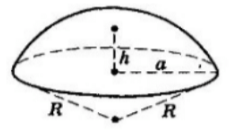
\includegraphics[width=0.1\textwidth]{content/mathematics/ball-segment.png}
\end{center}

\[\begin{array}{cc}
  a = \sqrt{h \cdot (2R - h)}\\
  V = \pi \cdot h^2(R -\frac{h}{3})
\end{array}\]

\begin{center}
  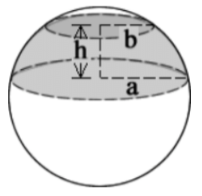
\includegraphics[width=0.1\textwidth, center]{content/mathematics/ball-layer.png}
\end{center}

\[\begin{array}{cc}
  V = \frac{1}{6}\pi h(3a^2+3b^2+h^2)\\
  R = \sqrt{\frac{((a - b)^2 + h^2)((a + b)^2 + h^2)}{4h^2}}
\end{array}\]  

\section*{Triangle formulas}
\begin{align*}
S &= \sqrt{p(p - a)(p - b)(p - c)} = \frac{abc}{4R}\\
m_a^2 &= \frac{2b^2 + 2c^2 - a^2}{4} \text{(median)}\\
w_a^2 &= \frac{bc((b + c)^2 - a^2)}{(b + c)^2} \text{(bisector)}\\
\frac{a}{\sin A} &= \frac{b}{\sin B} = \frac{c}{\sin C} = 2R\\
a^2 &= b^2 + c^2 - 2bc\cos A
\end{align*}

\section*{Monge's theorem}
There are three circles(balls) of different radii, 
for each pair of circles find the point of intersection of the external tangents. 
All three obtained points \textbf{lie on a line}. 
The point from the pair of the largest and the smallest \textbf{lies between} the other two.

\begin{center}
  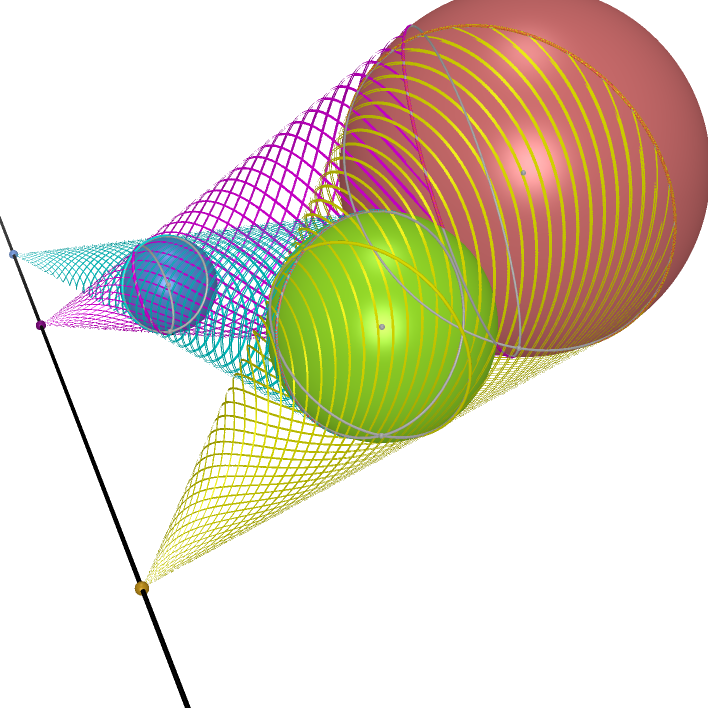
\includegraphics[width=0.15\textwidth, center]{content/mathematics/monges-theorem.png}
\end{center}

\section*{Pick's theorem}
Suppose that a polygon has integer coordinates for all of its vertices. 
Let $i$ be the number of integer points inside, and let $b$ be the number of integer points on boundary. 
Then the area $S = i + \tfrac{b}{2} - 1$.

\section*{Ptolemy's theorem}
For a general quadrilateral $ABCD$ holds:
$AB \cdot CD + AD \cdot BC \ge AC \cdot BD$.

Equality holds if and only if the quadrilateral is cyclic.

\section*{Euler line}
For a general triangle, the orthocenter $H$, the centroid $G$, 
and the circumcenter $O$, in this order, lie on the same line (Euler line) 
and $\frac{|HG|}{|GO|} = \frac{2}{1}$.

\section*{Fermat point}

In a given triangle $\triangle ABC$ the Fermat point is the point $X$,
which minimizes the sum of distances from $A$, $B$, and $C$,
$|AX| + |BX| + |CX|$.

If all angles of the triangle are less than $120^\circ$,
the the Fermat point is the interior point $X$
from which each side subtends an angle of $120^\circ$, i.e., 
$\angle BXC = \angle CXA = \angle AXB = 120^\circ$.

If any angle of the triangle formed by those points is $120^\circ$ or more,
then the Fermat point is the vertex of that angle.
